\chapter{Обзор предметной области}

Чтобы достичь намеченных целей, необходимо понять, что из себя представляет экран мобильного приложения, а также из каких элементов может состоять его интерфейс.

\section{Основные понятия}
В iOS существует различие между координатами, указываемыми в коде, и пикселями устройства -- наименьшими дискретными элементами двумерного цифрового изображения \cite{pixel}. Для большинства задач фактический размер точек \cite{point} не имеет значения, их цель -- обеспечить согласованный масштаб, который может использоваться в коде для указания размера и положения представлений и отображаемого содержимого. Например, если пиксели в два раза меньше изначальной высоты или ширины, можно использовать квадрат 2×2 пикселя для каждой точки (это называется масштаб @2x). Таким образом, измерение в точках позволяет корректно масштабировать изображение на экранах с высоким разрешением. \cite{hig}

\begin{figure}[h!]
	\centering{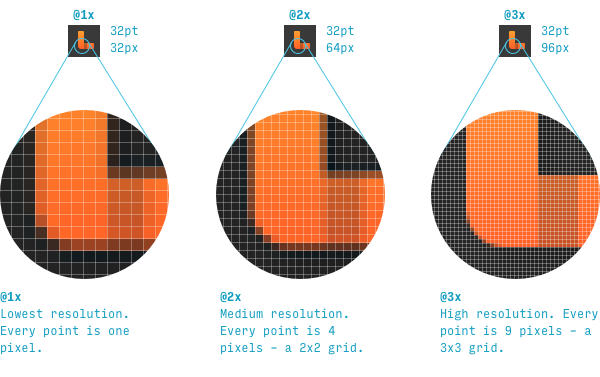
\includegraphics[scale=0.75]{img/point.png}}
	\caption{Точки и пиксели}
	\label{fig:points}
\end{figure}

Устройства, работающие на операционной системе iOS, имеют различное разрешение экрана и соотношение сторон. Так, например, iPhone X имеет разрешение 1125 x 2436 пикселей и коэффициент масштабирования в точки, равный 3.0 (то есть 375 x 812 точек), а iPhone 6  -- 750 x 1334 пикселей и коэффициент 2.0 соответственно (то есть 375 x 667). Данные характеристики стоит учитывать в разработке, дабы создавать приложения, интерфейс которых адаптируется к устройствам разного размера. 

\section{UIKit}

UIKit -- библиотека, предоставляющая архитектуру окон и представлений для реализации пользовательского интерфейса, включая компоненты, которые можно использовать для построения базовой инфраструктуры приложения \cite{uikit}. Альтернативой выступает фреймворк SwiftUI \cite{swiftui}, предоставляющий не меньше возможностей, однако, будучи представленным в 2016 году, библиотека не смогла стать столь популярной в разработке. Поэтому целесообразным будет рассмотреть методы верстки UI-элементов, предоставляемых UIKit.


Рассмотрим базовые UI-элементы, предоставляемые фреймворком UIKit.

UIView (или представление) -- это фундаментальный блок пользовательского интерфейса приложения, а UIView-класс определяет поведение, общее для всех представлений \cite{uiview}. Объекты этого класса отображают содержимое в пределах своих границ и обрабатывают любые взаимодействия с этим содержимым. Для отображения надписей, изображений, кнопок и других элементов интерфейса, обычно встречающихся в приложениях, используют не определяемые самостоятельно подклассы view, а предоставляемые платформой UIKit. 

UIViewController (или контроллер) -- объект, который управляет иерархией представлений приложения \cite{controller}. Основные обязанности контроллера включают следующее:

\begin{itemize}
	\item обновление содержимого представлений;
	\item реагирование на взаимодействие пользователя с представлениями;
	\item изменение размеров представлений и управление макетом общего интерфейса;
	\item координация с другими объектами, включая другие контроллеры представления.
\end{itemize}

Итак, экран в мобильной разработке представляет UIViewController, являющийся контейнером для других UIView. Труд команды разработки интерфейса мобильного приложения сводится к задаче корректного отображения элементов на экране -- расположения UIView на UIViewController. Чтобы работа была эффективной, целесообразно каждому члену команды дать индивидуальную подзадачу -- таким образом используемая технология верстки должна предполагать возможность работы нескольких участников над одним проектом и минимизировать количество ошибок, возникающих при изменении параметров UI-элементов. 

На основе рассмотренных теоретических сведений можно выделить критерии, по которым необходимо провести анализ эффективности использования методов верстки:

\begin{itemize}
	\item возможность создания масштабируемого для разных устройств интерфейса и относительная сложность его создания;
	\item относительная сложность командной разработки интерфейса;
	\item относительная сложность внесения изменений в интерфейс;
	\item порог входа в технологию метода и ее наглядность; ???
	\item возможность обработки всех параметров UI-элемента;
	\item скорость работы метода.
\end{itemize}

Рассматривать разные элементы?

\chapter{Методы верстки}

Существует три основных подхода к созданию пользовательского интерфейса: можно программно компоновать пользовательский интерфейс с помощью, использовать маски автоматического изменения размера, чтобы автоматизировать некоторые реакции на внешние изменения, или использовать автоматическую компоновку.
\section{Ручная верстка}
\subsection{Frame}

\section{Автоматическая верстка}
\subsection{Storyboard}
\subsection{Xib}
\subsection{Auto Layout}
